\documentclass[titlepage=firstiscover, captions=tableheading, bibliography=totoc]{scrartcl}
\usepackage[autostyle=true,german=quotes]{csquotes}
\usepackage{scrhack}
\usepackage{caption}
\usepackage[aux]{rerunfilecheck}
\usepackage{subcaption}        
\usepackage{fontspec}
\usepackage[dvips]{graphicx}
\usepackage{floatflt,epsfig} 
    
\usepackage{polyglossia}
\setmainlanguage{german}

\usepackage[unicode]{hyperref}
\usepackage{bookmark}
\title{V27\\ Der Helium-Neon-Laser}
\author{
Miriam Simm\\
\texorpdfstring{\href{mailto:miriam.simm@tu-dortmund.de}{miriam.simm@tu-dortmund.de}\and}{,}
Katrin Bolsmann\\
\texorpdfstring{\href{mailto:katrin.bolsmann@tu-dortmund.de}{katrin.bolsmann@tu-dortmund.de}}{}
}
\date{Durchführung: 15.06.2020 \\ Abgabe: -.06.2020}
\usepackage{amsmath} 
\usepackage{amssymb} 
\usepackage{mathtools}
\usepackage[
    math-style=ISO,
    bold-style=ISO,
    sans-style=italic,
    nabla=upright,
    partial=upright,
]{unicode-math}
    
\setmathfont{Latin Modern Math}

\usepackage[
  locale=DE,
  separate-uncertainty=true, 
  per-mode=symbol-or-fraction,
]{siunitx}

\usepackage{multicol}
\setlength{\columnsep}{1pt} %space between columns 

\usepackage{booktabs}
\usepackage[x11names, table]{xcolor}
\usepackage{graphicx}
\usepackage{grffile}
\usepackage{xfrac}
\usepackage{xcolor}

\usepackage{float}
\floatplacement{figure}{h}
\floatplacement{table}{h}
\usepackage[
  section,
  below,
]{placeins}

\usepackage{expl3}
\usepackage{xparse}
\ExplSyntaxOn
\NewDocumentCommand \E {} {\symup{e}}
\ExplSyntaxOff

% Literaturverzeichnis
\usepackage[
  backend=biber,
]{biblatex}
% Quellendatenbank
\addbibresource{literatur.bib}

\usepackage[
  version=4,
  math-greek=default,
  text-greek=default,
]{mhchem}
 

\raggedcolumns

\begin{document}

\maketitle

\section{Zielsetzung}
Ziel des Versuchs ist die Untersuchung der Funktionsweise eines Helium-Neon-Lasers, sowie der Einfluss 
der einzelnen Elemente auf seine Funktion.
%lol ich bin mir bei dem Satz nicht so sicher

\section{Theorie}
Ein Laser erzeugt monochromatisches Licht hoher Intensität und Kohärenz und findet in vielen technischen 
und wissenschaftlichen Bereichen Anwendung.
Prinzipiell besteht ein Laser aus drei Komponenten: einem aktiven Lasermedium, 
einer Pumpquelle und einem Resonator. 
Im aktiven Medium, welches das Spektrum der emittierten Strahlung bestimmt, 
entstehen Photonen durch optische Übergänge angeregter Atome. Zur Erzeugung der dafür notwendigen Besetzungsinversion 
führt die Pumpquelle dem Medium permanent Energie zu.
Der Resonator besteht aus zwei gegenüberliegenden Spiegeln, an denen Photonen reflektiert werden. Dadurch durchlaufen
diese mehrmals das aktive Medium, wodurch neue Photonen emittiert werden und ein selbsterregender Oszillator entsteht.
%Im aktiven Medium werden durch einen optischen Übergang Photonen erzeugt

\subsection*{Optische Übergänge}
Bei den optischen Übergängen zwischen den diskreten Energieniveaus $E_1$ und $E_2$ in den Atomen des aktiven Mediums
müssen die drei Fälle Absorption, spontane Emission und induzierte Emission unterschieden werden. Diese sind in 
Abbildung \ref{fig:tfig1} schematisch dargestellt.
\FloatBarrier
    \begin{figure}[h]
    \centering
    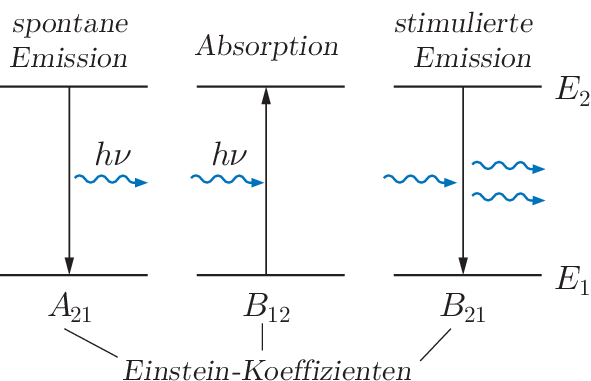
\includegraphics[width=0.6\textwidth]{optisch.png}
    \caption{Optische Übergänge im Zwei-Niveau-System \cite{quelle05}.}
    \label{fig:tfig1}
    \end{figure}
\FloatBarrier
\noindent
Es wird nun ein vereinfachtes Modell mit zwei Niveaus mit Besetzungszahlen $n_1$ und $n_2$ betrachtet. 
%Vereinfacht werden nur zwei Niveaus mit Besetzungszahlen $n_1$ und $n_2$ betrachtet. 
Absorption tritt auf, wenn ein einfallendes Photon genau die Energie des Übergangs besitzt. Das Photon wird dann von einem
Elektron absorbiert, welches dadurch in ein höheres Energieniveau angeregt wird.
Bei spontaner Emission findet ein Übergang eines Elektrons in ein niedrigeres Energieniveau statt. Die dabei freiwerdende
Energie wird in Form eines Photons emittiert. Geschieht dieser Übergang nicht spontan, sondern wird von einem einfallenden 
Photon herbeigeführt, so findet induzierte Emission statt. Das emittierte und das einfallende Photon haben dann die gleiche
Energie, Phase und Ausbreitungsrichtung.

Eine Verstärkung des Lichts im Laser wird erreicht, wenn stimulierte Emission häufiger auftritt als spontane Emission, 
da sich dadurch die Anzahl der Photonen jeweils verdoppelt und eine hohe Verstärkung erreicht wird. 
Dazu muss das energetisch höhere Niveau stärker besetzt sein als das energetisch niedrigere. Für diese
Besetzungsinversion wird dem aktiven Medium mit der Pumpquelle ständig Energie zugeführt, wodurch die Besetzungswahrscheinlichkeit
des höheren Niveaus steigt. 

Im hier beschriebenen Zwei-Niveau-System ist es jedoch gar nicht möglich, die Besetzungsinversion zu realisieren.
Der Pumpvorgang findet hier direkt zwischen den beiden Niveaus statt, wodurch die Besetzung des oberen Niveaus zwar erhöht wird,
aufgrund der kurzen Relaxationszeit durch spontane Emission jedoch auch unmittelbar wieder absinkt, sodass 
maximal eine Gleichbesetzung beider Niveaus erreicht werden kann.

Notwendig ist daher ein weiteres Energieniveau $E_3$. Der Pumpvorgang findet nun zwischen $E_1$ und $E_3$ statt.
Ist der Übergang $E_3 \rightarrow E_2$ deutlich schneller als der Übergang $E_2 \rightarrow E_1$, 
kann eine höhere Besetzung von $E_2$ als von $E_1$ erreicht werden.
%sodass der Pumpvorgang zwischen $E_1$ und $E_3$ stattfindet. Wichtig ist,
%dass der Übergang $E_3 \rightarrow E_2$ deutlich schneller ist als der Übergang $E_2 \rightarrow E_1$.
%Dann ist jedoch die Wahrscheinlichkeit, dass ein Photon von einem Atom im oberen 
%Niveau durch stimulierte Emission abgegeben wird gleich der Wahrscheinlichkeit, dass ein Atom im unteren Niveau ein 
%Photon absorbiert. Spontane Emission führt dann dazu, dass das obere Niveau immer weniger besetzt ist als das untere.


\subsection*{Optischer Resonator}
Die Verstärkung des Lichts wächst exponentiell mit dem Laufweg durch das aktive Medium an, weswegen mit dem 
Resonator dieser Laufweg verlängert wird. Der Resonator besteht aus zwei gegenüberliegenden Spiegeln, von denen einer, der Auskoppelspiegel, 
halbdurchlässig ist. Zwischen diesen Spiegeln wird das Licht reflektiert und durchläuft daher das aktive Medium mehrmals.
%wie in Abbildung \ref{fig:tfig2} dargestellt.
%\FloatBarrier
%    \begin{figure}[h]
%    \centering
%    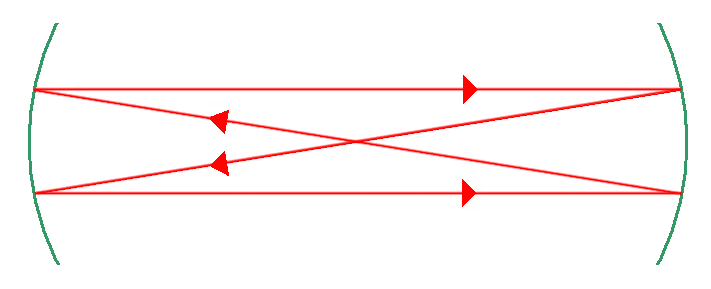
\includegraphics[width=0.6\textwidth]{strahlen.png}
%    \caption{Strahlenverlauf im Resonator des Lasers zwischen zwei konkaven Spiegeln \cite{quelle06}.}
%    \label{fig:tfig2}
%    \end{figure}
%\FloatBarrier
%\noindent
Für die einzelnen Spiegel können dabei sowohl planparallele als auch sphärische Spiegel eingesetzt werden. 
Selbsterregende Oszillation tritt ein, wenn die Verluste im Resonator kleiner sind als die Verstärkung durch 
induzierte Emission. Das ist der Fall, wenn die Stabilitätsbedingung
\begin{equation}
    \label{eq:stabil}
    0 \leq g_1 \cdot g_2 \leq 1 
\end{equation}
mit den Stabilitätsparametern $g_i = 1 - \frac{L}{r_i}$ erfüllt ist, wobei $r_i$ der Krümmungsradius des Spiegels
und $L$ die Resonatorlänge ist.
Wie in Abbildung \ref{fig:tfig3} erkennbar, hat $g_1 \cdot g_2$ eine Nullstelle, wenn die Länge des Resonators
genau dem Krümmungsradius eines Spiegels entspricht.
\FloatBarrier
    \begin{figure}[h]
    \centering
    \includegraphics[width=0.8\textwidth]{g1g2.pdf}
    \caption{Verlauf von $g_1 \cdot g_2$ in Abhängigkeit von der Länge $L$ des Resonators.}
    \label{fig:tfig3}
    \end{figure}
\FloatBarrier
\noindent

\subsection*{Resonatormoden}
Da die Länge des Resonators deutlich über der Wellenlänge des Laserlichts liegt, erfüllen viele Wellenlängen die 
Resonanzbedingung 
\begin{equation*}
    2 L = q \cdot \lambda 
\end{equation*}
und erzeugen eine stehende Welle zwischen den Resonatorspiegeln. Die Anzahl $q$ dieser Wellenlängen ist die longitudinale
Mode. Durch störende Einflüsse wie Verkippungen der Spiegel können auch transversale Moden auftreten.
%, die Verteilung der Phasenlage der Wellen senkrecht zur Ausbreitungsrichtung. 
Die Moden eines Lasers werden mit $TEM_{lpq}$ gekennzeichnet, wobei $TEM$ abkürzend für \textit{Transverse Electric Mode} ist
und $l$ und $p$ die Knoten in $x$- und $y$-Richtung sind und als transversale Modenzahl bezeichnet werden.
Die Grundmode ohne Knoten in transversaler Richtung ist die $TEM_{00}$ Mode. Ihre Intensität folgt einer
Gaußverteilung mit der Leistung
\begin{equation*}
    \symup{\Phi} \left(r\right) = \symup{\Phi}_0 \text{e}^{-\frac{2 r^2}{\omega^2}} \, ,
\end{equation*}
mit der Maximalintensität $\symup{\Phi}_0$, dem dem Abstand zur optischen Achse $r$ und dem Strahlradius $\omega$
\begin{equation*}
    \omega \left(z\right) = \sqrt{1 + \left(\frac{\theta z}{\omega_0}\right)} \, .
\end{equation*}
Hierbei ist $\omega_0$ die minimale Strahlweite im Abstand $z$ und $\theta = \frac{\lambda}{\pi} \omega_0$ die Strahldivergenz.

Die Intensitätsverteilung der $TEM_{m,n}$-Mode bei $z = 0$ ist ein Produkt aus zwei Hermite-Polynomen und einer Gaußfunktion
\begin{equation*}
    I\left(x, y\right) = I_0 H_m \left(\frac{\sqrt{2} x}{\omega}\right) H_n \left(\frac{\sqrt{2} y}{w}\right)\cdot \text{e}^{- \frac{x^2 + y^2}{\omega^2}} \, .
\end{equation*}
Die Verteilungsfunktion der Intensität der $TEM_{01}$-Mode ist daher
\begin{equation}
    \label{eq:kermit}
    I\left(x, y\right) = I_0 H_0 \left(\frac{\sqrt{2} x}{\omega}\right) H_1 \left(\frac{\sqrt{2} y}{w}\right)\cdot \text{e}^{- \frac{x^2 + y^2}{\omega^2}} \, ,
\end{equation}
mit der Leistung
\begin{equation*}
    \symup{\Phi} \left(x, y\right) = \symup{\Phi}_0 H_0 \left(\frac{\sqrt{2} x}{\omega}\right) H_1 \left(\frac{\sqrt{2} y}{w}\right)\cdot \text{e}^{- \frac{x^2 + y^2}{\omega^2}}
\end{equation*}

\subsection*{Das Brewster-Fenster}
Ein Brewster-Fenster ist ein Polarisator, der sehr verlustarm ist, und sich daher gut für einen Laser eignet.
Dazu befindet sich das Fenster im Brewster-Winkel zur optischen Achse. Wenn Licht im Brewster-Winkel auf eine Grenzfläche
trifft, werden nur die zur Einfallsebene senkrechten Anteile reflektiert, sodass das reflektierte Licht linear polarisiert 
ist. Mit dem Brewster-Fenster kann daher parallel polarisiertes Lichts sehr verlustarm in die Helium-Neon-Röhre ein- und aus ihr wieder austreten.

\subsection*{Der Helium-Neon-Laser}
Das Laserrohr ist mit einem Gasgemisch aus Helium und Neon gefüllt, wobei das Verhältnis von Helium zu Neon 5:1 beträgt.
Das Heliumgas dient als Pumpquelle und das Neongas als aktives Medium. Im Laserrohr befinden sich Elektroden, sodass 
Gasentladungen stattfinden. Diese regen die Heliumatome in einen metastabilen Zustand an, die dann ihre Energie auf 
die Neonatome übertragen
\begin{equation*}
    \text{He}^{*} + \text{Ne} \rightarrow \text{He} + \text{Ne}^{*} + \Delta E \, .
\end{equation*}
Das Niveauschema des Helium-Neon-Lasers ist in Abbildung \ref{fig:tfig8} dargestellt.
Der Übergang $3s_2 \rightarrow 2p_4$ erzeugt die rote Laserlinie bei $632.8 \, \si{\nano\meter}$.
\FloatBarrier
    \begin{figure}[h]
    \centering
    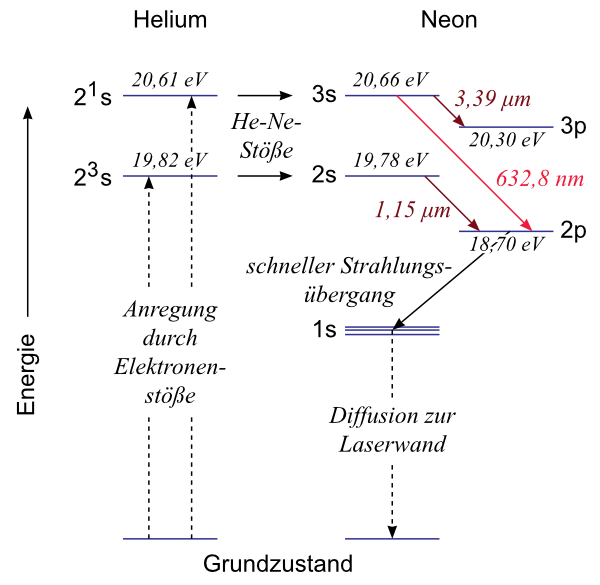
\includegraphics[width=0.5\textwidth]{henelaser.png}
    \caption{Niveauschema Helium-Neon-Lasers \cite{quelle01}.}
    \label{fig:tfig8}
    \end{figure}
\FloatBarrier
\noindent
Mit einem Gitter kann über Interferenz die Wellenlänge des Lasers bestimmt werden. Aus der Beugungsbedingung 
\begin{equation*}
    n \lambda = a \cdot \sin \left(\theta \right)
\end{equation*}
folgt für die Wellenlänge
\begin{equation}
    \label{eq:Wellenlänge}
    \lambda = \frac{a}{n}  \sin \left(\arctan \left(\frac{d}{L}\right)\right)     \, ,
\end{equation}
mit dem Abstand der Gitterelemente $a$, der Ordnung $n$ des Maximums, dem Abstand $d$ des Maximums vom 0. Hauptmaximum
und dem Abstand $L$ vom Gitter zum Schirm.

\section{Aufbau}
Der Aufbau des Versuchs ist in Abbildung \ref{fig:dfig1} dargestellt. Die einzelnen Elemente des Lasers befinden sich 
auf einer optischen Schiene, sodass die Spiegel beliebig verstellt werden können. 

Zur Justage ist im Aufbau ein weiter Laser der Wellenlänge $\lambda = 532 \, \si{\nano\meter}$ mit reduzierter 
Laserleistung ($P_\text{red} = 0.2 \, \si{\milli\watt}$) integriert. Dessen Licht durchläuft eine Blende, auf deren Rückseite sich ein Fadenkreuz befindet, 
dass zum genauen Einstellen des Helium-Neon-Lasers verwendet wird.
Der Helium-Neon-Laser besteht aus zwei Resonatorspiegeln mit konkaver Krümmung und Durchmesser $d = 12.7 \, \si{\milli\meter}$ und einem Laserrohr.
Der Krümmungsradius der Spiegel beträgt $r = 1400 \, \si{\milli\meter}$. Das Laserrohr mit Länge $L = 408 \, \si{\milli\meter}$
und Durchmesser $d = 1.1 \, \si{\milli\meter}$ ist mit einem Gemisch aus Helium- und Neongas gefüllt. An seinen Enden 
befinden sich zwei Brewster-Fenster.
\FloatBarrier
    \begin{figure}[h]
    \centering
    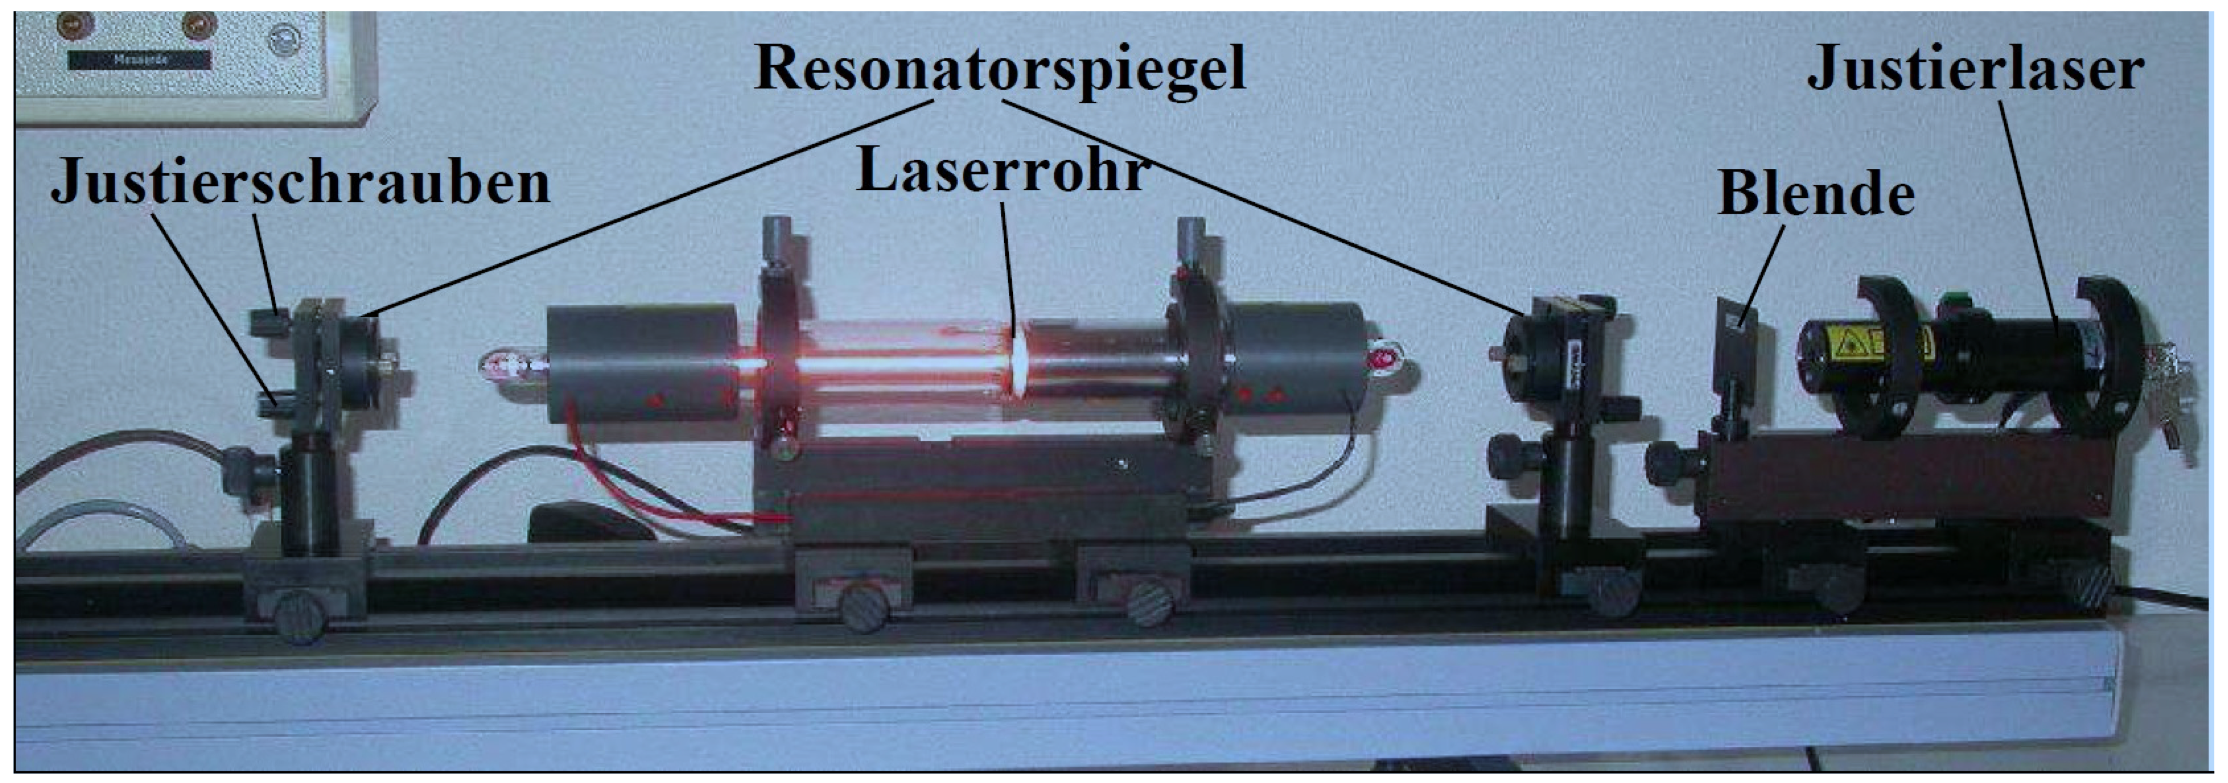
\includegraphics[width=\textwidth]{aufbau.png}
    \caption{Aufbau des verwendeten Helium-Neon-Lasers \cite{quelle01}.}
    \label{fig:dfig1}
    \end{figure}
\FloatBarrier
\noindent
Zur Untersuchung der Funktionsweise des Laser können außerdem eine Photodiode, ein Polarisator und ein Schirm
in den Strahlengang eingebracht werden. 

\section{Durchführung}
Vor Beginn der Messung wird der Laser justiert. Für die Besetzungsinversion zu erzeugen, ist an den Elektroden des
Laserrohrs ein Strom von $6.52 \, \si{\milli\ampere}$ angelegt.
Dann wird zuerst zur Bestimmung der Polarisation ein Polarisator in den Strahlengang eingebracht. Mit einer Photodiode
wird die Leistung des Lasers in Abhängigkeit von der Polarisationsrichtung gemessen, wobei der Polarisator in
10°-Schritten verstellt wird. 
Außerdem wird die Nullleistung bei ausgeschaltetem Laser gemessen.

Anschließend wird die Stabilitätsbedingung überprüft. Dazu wird der Abstand der Resonatorspiegel in $2 \, \si{\centi\meter}$-Schritten
variiert und ebenfalls die Leistung gemessen. 
Außerdem wird die $\text{TEM}_{00}$-Mode vermessen, wozu eine Streulinse in den Aufbau integriert wird, die den Laserstrahl vergrößert.
Mit einer Blende, die in $2 \, \si{\milli\meter}$-Schritten verschoben wird, wird jeweils ein kleiner Teil des Lichts 
herausgefiltert, dessen Strahlungsleistung gemessen wird. 

Zur Untersuchung der $\text{TEM}_{01}$-Mode wird zusätzlich sowohl ein dünner Draht als auch ein Haar in den Strahlengang gebracht.
%Ich weiß nicht ob der Satz so reicht aber ich will jetzt irgendwie auch nicht so halb hier schon die Diskussion schreiben :D
Nach dieser Messung werden drei verschiedene Gitter mit Gitterkonstanten $d = 100 \, \text{Linien} / \si{\milli\meter}$, $d = 600 \, \text{Linien} / \si{\milli\meter}$ und $d = 1200 \, \text{Linien} / \si{\milli\meter}$
in den Strahlengang eingebracht. Um die Wellenlänge des Lasers bestimmen zu können, wird das Beugungsbild 
auf einem Schirm abgebildet und jeweils der Abstand zum Hauptmaximum sowie der Abstand von Schirm und Gitter gemessen.

\section{Auswertung}
\subsection{Überprüfung der Stabilitätsbedingung}
Die Messwerte zur Überprüfung der Stabilitätsbedingung sind in der Tabelle \ref{tab:atab1} des Anhangs zu finden.
Nach \eqref{eq:stabil} zeigt die Leistung für zwei konkave Spiegel $r=1400\,\si{\mm}$ einen quadratischen Verlauf, somit werden die Messwerte an eine quadratische Funktion der Form
\begin{equation}
    \symup{\Phi}(L) = a L^2 + b L + c \label{eq:fit1}
\end{equation}
gefittet. 
Um die Messwerte besser vergleichen zu können werden diese normiert und die Nullleistung, für welche ein Wert von $\symup{\Phi} = (16.63 \pm 0.04) \, \si{\micro\W}$ gemessen wurde, abgezogen.
Die entsprechenden Fitparameter sind in Tabelle \ref{tab:atab2} zu finden, wobei zurerst die Messreihen separat und anschließend alle Messwerte zusammen betrachtet werden. 
Die Messdaten und die nach \eqref{eq:fit1} errechneten Ausgleichspolynome sind in den Abbildungen \ref{fig:afig1} und \ref{fig:afig2} dargestellt.
Eine ausführliche Diskussion der Plots ist in Abschnitt \ref{sec: Diskussion} zu finden.

Diese und alle folgenden Ausgleichsrechnungen werden mit dem Paket 
$\texttt{SciPy.optimize.curve\_fit}$ durchgeführt. 
Fehlerrechnung erfolgt mittels dem $\texttt{Python}$-Paket $\texttt{uncertainties.unumpy}$.
\FloatBarrier
\begin{table}[h]
    \centering
    \caption{Parameter der Gleichung \eqref{eq:fit1}.}
    \label{tab:atab2}
    \begin{tabular}{l c c c c}
        \toprule
        {} & {Messung 1} & {Messung 2} & {Messung 3} & {alle Messwerte} \\
        \midrule
        $a / \si{\micro\W\per\cm\squared}\cdot10^{3}$ & $(1,1 \pm 0,7)$ & $(0,2 \pm 0,8)$ & $(1,5 \pm 0,4)$ & $(0,5 \pm 0,4)$ \\
        $b / \si{\micro\W\per\cm}\cdot10^{2}$ & $(-20 \pm 12)$ & $(-6 \pm 14)$ & $(-26 \pm 6)$ & $(-10 \pm 6)$ \\
        $c / \si{\micro\W}$ & $(9 \pm 5)$ & $(5 \pm 6)$ & $(11,5 \pm 2,3)$ & $(5,2 \pm 2,5)$ \\
        \bottomrule
    \end{tabular}
\end{table}
\FloatBarrier
\noindent
\FloatBarrier
\begin{figure}[h]
\centering
\includegraphics[width=\textwidth]{Stabilität.pdf}
\caption{Messwerte der Strahlungsleistung aller drei Messreihen in Abhängigkeit der Resonatorlänge und Ausgleichsrechnung für $r_1=r_2=1400\,\si{\mm}$.}
\label{fig:afig1}
\end{figure}
\FloatBarrier
\noindent
\FloatBarrier
\begin{figure}[h]
\centering
\includegraphics[width=\textwidth]{Stabilität_all.pdf}
\caption{Messwerte der Strahlungsleistung in Abhängigkeit der Resonatorlänge und Ausgleichsrechnung $r_1=r_2=1400\,\si{\mm}$.}
\label{fig:afig2}
\end{figure}
\FloatBarrier
\noindent

\subsection{Untersuchung der TEM-Moden}
Die Messdaten zur Untersuchung der $\text{TEM}_{0,0}$-Mode sind in Tabelle \ref{tab:atab3} des Anhangs zu finden. 
Die Grundmode wird an eine Gaußfunktion der Form
\begin{equation}
\symup{\Phi}(x) = \symup{\Phi}_0 \text{exp}\left(-2\left(\frac{(x-x_0)}{\omega}\right)^2\right) \label{eq:fit2}
\end{equation}
gefittet. 
Dabei stellt $\symup{\Phi}_0$ die maximale Strahlungsleistung und $x_0$ die transversale Verschiebung des Maximums dar. 
$\omega$ ist ein Maß für die Breite der Verteilung. 
Für diese drei freien Parameter ergeben sich die Werte
\begin{align}
\symup{\Phi}_0 &= (22,5 \pm 0,9)\,\si{\micro\watt} \\
x_0 &= (12,2 \pm 1,2)\,\si{\mm}\\
\omega &= (26\pm6)\,\si{\mm} \quad .
\end{align}
Die daraus resultierende Ausgleichsfunktion ist zusammen mit den Messwerten in Abbildung \ref{fig:afig3} aufgetragen.
\noindent
\FloatBarrier
\begin{figure}[h]
\centering
\includegraphics[width=\textwidth]{TEM00.pdf}
\caption{Messdaten der Strahlungsleistung der $\text{TEM}_{0,0}$-Mode entlang der transversalen Achse sowie der Gaußfunktion \eqref{eq:fit2}.}
\label{fig:afig3}
\end{figure}
\FloatBarrier

\subsection{Untersuchung der Polarisation}
Die für die Polarisationsuntersuchung aufgenommenen Messwerte sind in Tabelle \ref{tab:atab4} des Anhangs zu finden. 
In Abbildung \ref{fig:afig4} ist die Strahlungsleistung gegen den Winkel $\alpha$ des Polarisationsprismas aufgetragen.
\noindent
\FloatBarrier
\begin{figure}[h]
\centering
\includegraphics[width=\textwidth]{Polarisation.pdf}
\caption{Sinusförmiger Verlauf der Strahlungsleistung in Abhängigkeit der Winkels des Polarisationsprismas.}
\label{fig:afig4}
\end{figure}
\FloatBarrier
Die Ausgleichsfunktion hat die Form
\begin{equation}
\symup{\Phi}(\alpha) = \symup{\Phi}_0 \sin^2{\alpha-\alpha_0} \quad ,
\end{equation}
wobei sich für die freien Parameter die Werte
\begin{align}
\symup{\Phi}_0 & = (790\pm 6)\, \si{\micro\watt}\\
\alpha_0 &= (-0,353\pm 0,007)\, \mathrm{rad}
\end{align}
ergeben. 
Die Minimalleistung ist demnach bei einem Winkel von
\begin{align}
\alpha - \alpha_0 &= 2\pi n \qquad \qquad n \in \mathbb{N} \\
\Leftrightarrow \qquad \quad \alpha &=  2\pi n + \alpha_0 \\
&\stackrel{n = 0}{=} (-0,353\pm 0,007)\, \mathrm{rad} \\
&= -20.2° \pm 0.4°
\end{align}
erreicht. Somit folgt, dass das Licht des HeNe-Laser linear in einer um $-20,2°$ gekippten Ebene polarisiert ist.

\subsection{Berechnung der Wellenlänge}
Die Wellenlänge wird anhand des Interferenzmusters, welches sich durch Beugung an einem Gitter ergibt, errechnet.
Hierzu wurden drei Gitter mit unterschiedlichen Liniendichten betrachtet.
Die Messwerte sind in Tabelle \ref{tab:atab5} des Anhangs zu finden. 
Hierbei beschreibt $n$ jeweils die Ordnung des Hauptmaximums, also um das wievielte Maximum ausgehend vom zentralen Maximum es sich handelt.

Die Wellenlänge wird mittels der Formel \eqref{eq:Wellenlänge} berechnet.
Somit ergibt sich für jedes vermessene Maximum ein Wert für die Wellenlänge, welche in Tabelle \ref{tab:atab6} angegeben sind.

\FloatBarrier
\begin{table}[h]
    \centering
    \caption{Nach \eqref{eq:Wellenlänge} berechneten Werte für die Wellenlänge aller drei Gitter.}
    \sisetup{table-format=2.1}
    \label{tab:atab6}
    \begin{tabular}{c c c c c c}
        \toprule
        \multicolumn{1}{c}{100 Linien/\si{\mm}} & \multicolumn{1}{c}{600 Linien/\si{\mm}} & \multicolumn{1}{c}{1200 Linien/\si{\mm}} \\
        \cmidrule(lr){1-1}\cmidrule(lr){2-2}\cmidrule(lr){3-3}
        {$\lambda /\si{\nm}$} & {$\lambda /\si{\nm}$} & {$\lambda /\si{\nm}$} \\
        \midrule
        643,2\pm 1,2 & 620,9 \pm 1,3 & 604,1 \pm 0,7 \\
        630,3\pm 1,1 & 624,8 \pm 0,7 & \\
        627,0\pm 1,1 & 633,5 \pm 1,3 & \\
        624,2\pm 1,1 & & \\
        626,2\pm 1,0 & & \\
        628,3\pm 1,0 & & \\
        628,5\pm 0,9 & & \\
        628,7\pm 0,9 & & \\
        630,3\pm 0,8 & & \\
        661,5\pm 1,2 & & \\
        630,3\pm 1,1 & & \\
        627,0\pm 1,1 & & \\
        628,3\pm 1,1 & & \\
        \\
        $\text{Mittelwerte}\,\bar{\lambda}/\si{\mm}$ & &\\
        \cmidrule(lr){1-1}\cmidrule(lr){2-2}\cmidrule(lr){3-3}
        631,8 \pm 1,1 & 626,4 \pm 1,1 & 604,1 \pm 0,7 \\
        \bottomrule
    \end{tabular}
\end{table}
\FloatBarrier
\noindent
Werden die Mittelwerte für die verschiedenen Gitter erneut gemittelt ergibt sich für die Wellenlänge ein Wert von
\begin{equation}
\lambda = (620,8 \pm 0,5) \, \si{\nm} \qquad .
\end{equation}


\section{Diskussion} \label{sec: Diskussion}
\subsection*{Überprüfung der Stabilitätsbedingung}
In diesem Versuch wurden für den Resonator zwei konkav gekrümmte Spiegel mit dem Radius $r=1400\,\si{\mm}$ verwendet.
Der erwartete Intensitätsverlauf ist demnach quadratisch im Abstand der Spiegel und besitzt ein Minimum bei $L = r$, in welchem die Intensität verschwindet.

In Abbildung \ref{fig:afig1} zeigen die Messwerte der 2. Messung entgegen der Erwartungen einen beinahe linearen Verlauf im beobachteten Bereich. 
Zwar ist bei den anderen beiden Messungen ein quadratischer Verlauf zu erkennen, jedoch weist keine der errechneten Ausgleichsfunktionen ein Minimum bei $L = 1,4\,\si{\m}$ auf.
Die Minima der 1. und 3. Messreihe liegen in einem Bereich zwischen $(0,85-0,95)\,\si{\m}$.

Die Ausgleichfunktion in Abbildung \ref{fig:afig2}, welche sich aus den Messwerten aller drei Messreihen ergibt, zeigt einen etwas besseren Verlauf.
Es ist ein Minimum bei circa $L=1,05\,\si{\m}$ zu erkennen, welches ein wenig näher an der Lage des erwarteten Minimums bei $L=1,40\,\si{\m}$ liegt.

Wahrscheinlich haben Fehler und Ungenauigkeiten bei dem Messprozessen zu diesen Abweichungen geführt.
Somit musste der HeNe-Laser bei Veränderung des Abstandes neu justiert werden und je nachdem wie gut der Laser justiert ist, schwankt die Strahlungsleistung stark.
Im Optimalfall wird immer die maximale Strahlungsleistung für die entsprechende Resonatorlänge gemessen, diese ist allerdings schwer zu erreichen.

Eine weitere Möglichkeit die Ergebnisse zu verbessern, wäre es mehr Messwerte vor allem für große Resonatorlängen zu nehmen.
Allerdings stellte sich die Messung für große Resonatorlängen ab etwa $1\,\si{m}$ als sehr schwierig dar, da aufgrund der geringen Leistung die Justage des Lasers kaum möglich war.


\subsection*{Untersuchung der TEM-Moden}
Die Grundmode konnte bei der Durchführung des Versuches auf dem Schirm sichtbar gemacht und somit vermessen werden. 
Jedoch ist in Abbildung \ref{fig:afig3} deutlich zu sehen, dass mehr Werte gerade in dem Bereich geringer Intensität hätten genommen werden müssen.

Ursprünglich ist auch die Vermessung der ersten angeregten Mode TEM$_{\text{01}}$ Teil dieses Versuches.
Für diese ist eine Intensitätsverteilung nach \eqref{eq:kermit} aus einer Gaußfunktion und dem ersten Hermite Polynom $H_1(x)$ zu erwarten.
Allerdings ist es auch nach etlichen Versuchen nicht gelungen diese auf dem Schirm sichbar zu machen.
Grund hier für könnte die Qualität des verwendetem Haares sein. 
Möglicherweise ist dieses bereits ein wenig ausgefranst oder anders beschädigt, sodass es sich nicht zur Unterdrückung von Moden eignet.


\subsection*{Untersuchung der Polarisation}
Die Messwerte zur Polarisationsuntersuchung zeigen genau den zu erwarteten $\sin^2$-Verlauf.
Dementsprechend repräsentiert die Ausgleichsfunktion diese Werte sehr gut und somit entspricht die Polarisationsrichtung dem berechneten Wert von $\alpha = -20.2° \pm 0.4°$ entspricht.

\subsection*{Berechnung der Wellenlänge}
Die berechneten Wellenlängen sind noch einmal in Tabelle \ref{tab:atab7} zusammengefasst und die Abweichung zu der tatsächlichen Wellenlänge eines Helium-Neon Lasers $\lambda = 632,8\,\si{\nm}$ angegeben.
\FloatBarrier
\begin{table}[h]
    \centering
    \caption{}
    \sisetup{table-format=2.1}
    \label{tab:atab7}
    \begin{tabular}{l c c}
        \toprule
        {} & {$\lambda /\si{\nm}$} & {Abweichung}\\
        \midrule
        100 Linien/\si{\mm} & 631,8 \pm 1,1 & 0,16\% \\
        600 Linien/\si{\mm} & 626,4 \pm 1,1 & 1,01\%\\
        1200 Linien/\si{\mm} & 604,1 \pm 0,7& 4,54\%\\
        \midrule
        Mittelwert & 620,8\pm 0,5 & 1,90\%\\ 
        \bottomrule
    \end{tabular}
\end{table}
\FloatBarrier
\noindent
Die Messung mit dem Gitter bei welchem der Linienabstand $0,01\,\si{\mm}$ beträgt, liefert das beste Ergebnis mit nur $0,16\%$ Abweichung vom realen Wert. 
Dies liegt wahrscheinlich daran, dass der Abstand der Maxima für geringe Liniendichten abnimmt. 
Somit konnten für das Gitter mit 100 Linien/$\si{\mm}$ die meisten Messwerte aufgenommen werden, während bei dem Gitter mit 1200 Linien/$\si{\mm}$ lediglich ein Abstand gemessen werden konnte.
Trotzdem liefern auch die anderen beiden Messungen sehr gute Werte mit jeweils Abweichungen von unter $5\%$.

\newpage
\appendix 
\section*{Anhang}\label{sec:Anhang}

\FloatBarrier
\begin{table}[h]
    \centering
    \caption{Messwerte der Strahlungsleistung $\symup{\Phi}$ in Abhängigkeit der Resonatorlänge $L$.}
    %\sisetup{table-format=2.1}
    \label{tab:atab1}
    \begin{tabular}{S[table-format=2.0]  S[table-format=4.2] @{}c @{}S[table-format=2.2] S[table-format=2.0] S[table-format=4.2] @{}c @{}S[table-format=2.2] S[table-format=2.0] S[table-format=4.2] @{}c @{}S[table-format=2.2]}
        \toprule
        \multicolumn{4}{c}{Messung 1} & \multicolumn{4}{c}{Messung 2} & \multicolumn{4}{c}{Messung 3} \\
        \cmidrule(lr){1-4}\cmidrule(lr){5-8}\cmidrule(lr){9-12}
        {$L/\si{\cm}$} & \multicolumn{3}{c}{$\symup{\Phi}/\si{\micro\W}$} & {$L/\si{\cm}$} & \multicolumn{3}{c}{$\symup{\Phi}/\si{\micro\W}$} & {$L/\si{\cm}$} & \multicolumn{3}{c}{$\symup{\Phi}/\si{\micro\W}$} \\
        \midrule
        %Hier bitte die Daten der Intensitäts-Abstands Messung einfügen aus den Intensität_Abstand txt dateien
        65 & 2360   &{$\;\pm\;$}&  14.89 & 72  & 1110   &{$\;\pm \;$}& 44.03 & 65 & 2510   &{$\;\pm \;$}& 10.66 \\  
        68 & 1820   &{$\;\pm\;$}&  14.36 & 74  & 588    &{$\;\pm \;$}& 39.78 & 67 & 1360   &{$\;\pm \;$}& 57.00 \\ 
        71 & 1170   &{$\;\pm\;$}&  34.68 & 76  & 924.27 &{$\;\pm \;$}& 44.73 & 69 & 1560   &{$\;\pm \;$}& 49.89 \\ 
        74 & 412.57 &{$\;\pm\;$}&  75.39 & 78  & 851.07 &{$\;\pm \;$}& 36.03 & 71 & 921.60 &{$\;\pm \;$}& 24.16 \\ 
        77 & 921.79 &{$\;\pm\;$}&  20.16 & 80  & 361.28 &{$\;\pm \;$}& 26.76 & 73 & 833.66 &{$\;\pm \;$}& 25.52 \\ 
        80 & 492.31 &{$\;\pm\;$}&  16.96 & 82  & 808.69 &{$\;\pm \;$}& 29.79 & 75 & 777.04 &{$\;\pm \;$}& 12.28 \\ 
        83 & 1120   &{$\;\pm\;$}&  18.82 & 84  & 730.28 &{$\;\pm \;$}& 19.44 & 77 & 316.69 &{$\;\pm \;$}& 22.79 \\ 
        86 & 174.23 &{$\;\pm\;$}&  20.99 & 86  & 705.03 &{$\;\pm \;$}& 15.69 & 79 & 712.24 &{$\;\pm \;$}& 36.35 \\ 
        89 & 616.18 &{$\;\pm\;$}&  40.15 & 88  & 100.47 &{$\;\pm \;$}& 12.66 & 81 & 326.80 &{$\;\pm \;$}& 19.74 \\ 
        92 & 102.00 &{$\;\pm\;$}&  28.61 & 90  & 343.30 &{$\;\pm \;$}& 27.88 & 83 & 186.66 &{$\;\pm \;$}& 26.16 \\ 
        95 & 85.79  &{$\;\pm\;$}&  36.63 & 92  & 115.33 &{$\;\pm \;$}& 21.93 & 85 & 488.59 &{$\;\pm \;$}& 68.30 \\ 
           &        &           &        & 94  & 52.01  &{$\;\pm \;$}& 16.49 & 87 & 214.32 &{$\;\pm \;$}& 13.42 \\
           &        &           &        & 96  & 64.43  &{$\;\pm \;$}& 8.9   & 89 & 508.34 &{$\;\pm \;$}& 96.39 \\
           &        &           &        & 98  & 201.34 &{$\;\pm \;$}& 8.09  & 91 & 332.00 &{$\;\pm \;$}& 30.45 \\
           &        &           &        & 100 &  51.65 &{$\;\pm \;$}& 7.20  & 93 & 185.48 &{$\;\pm \;$}& 34.34 \\
           &        &           &        &     &        &            &       & 95 & 287.22 &{$\;\pm \;$}& 20.12 \\
        \bottomrule
    \end{tabular}
\end{table}
\FloatBarrier
\noindent

\FloatBarrier
\begin{table}[h]
    \centering
    \caption{Messdaten der Strahlungsleistungs der $\text{TEM}_{0,0}$-Mode entlang der transversalen Achse.}
    %\sisetup{table-format=2.1}
    \label{tab:atab3}
    \begin{tabular}{S[table-format=2.0]  S[table-format=2.2] @{}c @{}S[table-format=1.2]}
        \toprule
        {$x/\si{\mm}$} & \multicolumn{3}{c}{$\symup{\Phi}/\si{\micro\W}$}\\
        \midrule
        % hier bitte die Messwerte der TEM Mode aus der datei TEM00_Mode.txt einfügen :)
        18 & 38.68 &{$\;\pm\;$}& 0.16 \\
        17 & 36.70 &{$\;\pm\;$}& 0.17 \\
        16 & 36.03 &{$\;\pm\;$}& 0.39 \\
        15 & 37.06 &{$\;\pm\;$}& 0.16 \\
        13 & 40.45 &{$\;\pm\;$}& 0.98 \\
        11 & 42.20 &{$\;\pm\;$}& 0.16 \\
        9  & 40.61 &{$\;\pm\;$}& 0.38 \\
        7  & 33.68 &{$\;\pm\;$}& 0.29 \\
        5  & 36.13 &{$\;\pm\;$}& 0.30 \\
        3  & 33.63 &{$\;\pm\;$}& 0.31 \\
        2  & 31.69 &{$\;\pm\;$}& 0.24 \\
        1  & 31.70 &{$\;\pm\;$}& 0.21 \\
        0  & 29.93 &{$\;\pm\;$}& 0.15 \\
        -1 & 30.42 &{$\;\pm\;$}& 0.25 \\
        -2 & 31.03 &{$\;\pm\;$}& 0.35 \\
        \bottomrule
    \end{tabular}
\end{table}
\FloatBarrier
\noindent

\FloatBarrier
\begin{table}[h]
    \centering
    \caption{Messwerte zur Untersuchung der Polarisation des HeNe-Lasers in Abhängigkeit des Winkels des Polarisationsprismas.}
    %\sisetup{table-format=2.1}
    \label{tab:atab4}
    \begin{tabular}{S[table-format=3.0]  S[table-format=3.2] @{}c @{}S[table-format=2.3]}
        \toprule
        {$\alpha/\mathrm{rad}$} & \multicolumn{3}{c}{$\symup{\Phi}/\si{\micro\W}$}\\
        \midrule
        % hier bitte die Messwerte der Polarisationsmessung aus der datei Polarisation.txt einfügen :)
        0    & 120.53 &{$\;\pm\;$}& 1.42 \\
        10   & 225.58 &{$\;\pm\;$}& 2.39 \\
        20   & 250.13 &{$\;\pm\;$}& 5.56 \\
        30   & 486.48 &{$\;\pm\;$}& 5.56 \\
        40   & 610.66 &{$\;\pm\;$}& 6.90 \\
        50   & 698.59 &{$\;\pm\;$}& 7.99 \\
        60   & 772.61 &{$\;\pm\;$}& 7.76 \\
        70   & 783.89 &{$\;\pm\;$}& 6.23 \\
        80   & 753.96 &{$\;\pm\;$}& 9.83 \\
        90   & 692.02 &{$\;\pm\;$}& 9.27 \\
        100  & 592.86 &{$\;\pm\;$}& 7.24 \\
        110  & 464.33 &{$\;\pm\;$}& 8.00 \\
        120  & 332.73 &{$\;\pm\;$}& 4.79 \\
        130  & 207.30 &{$\;\pm\;$}& 2.68 \\
        140  & 110.23 &{$\;\pm\;$}& 1.09 \\
        150  & 39.74  &{$\;\pm\;$}& 0.54 \\
        160  & 17.21  &{$\;\pm\;$}& 0.23 \\
        170  & 42.77  &{$\;\pm\;$}& 0.48 \\
        180  & 110.40 &{$\;\pm\;$}& 1.52 \\
        190  & 217.15 &{$\;\pm\;$}& 2.13 \\
        200  & 346.28 &{$\;\pm\;$}& 3.67 \\
        210  & 505.45 &{$\;\pm\;$}& 6.02 \\
        220  & 635.35 &{$\;\pm\;$}& 8.90 \\
        230  & 749.95 &{$\;\pm\;$}& 10.32 \\
        240  & 805.56 &{$\;\pm\;$}& 9.38 \\
        250  & 832.94 &{$\;\pm\;$}& 10.74 \\
        260  & 794.23 &{$\;\pm\;$}& 14.32 \\
        270  & 723.82 &{$\;\pm\;$}& 8.35 \\
        280  & 629.58 &{$\;\pm\;$}& 9.64 \\
        290  & 480.00 &{$\;\pm\;$}& 4.81 \\
        300  & 343.54 &{$\;\pm\;$}& 4.46 \\
        310  & 210.28 &{$\;\pm\;$}& 1.30 \\
        320  & 108.28 &{$\;\pm\;$}& 2.31 \\
        330  & 41.37  &{$\;\pm\;$}& 0.41 \\
        340  & 17.14  &{$\;\pm\;$}& 0.204 \\
        350  & 45.90  &{$\;\pm\;$}& 0.603 \\ 
        \bottomrule
    \end{tabular}
\end{table}
\FloatBarrier
\noindent

\FloatBarrier
\begin{table}[h]
    \centering
    \caption{Gemessene Abstände der Haupmaxima zum zentralen Hauptmaximum. Es wird eine Ablesefehler von $0,1\,\si{\cm}$ angenommen. $L$ ist der Abstand zwischen Gitter und Schirm.}
    %\sisetup{table-format=2.1}
    \label{tab:atab5}
    \begin{tabular}{S[table-format=1.0]  S[table-format=2.1] @{}c @{}S[table-format=1.1] S[table-format=1.0] S[table-format=2.1] @{}c @{}S[table-format=1.1] S[table-format=1.0] S[table-format=2.1] @{}c @{}S[table-format=1.1]}
        \toprule
        \multicolumn{4}{c}{100 Linien/\si{\mm}} & \multicolumn{4}{c}{600 Linien/\si{\mm}} & \multicolumn{4}{c}{1200 Linien/\si{\mm}} \\
        \multicolumn{4}{c}{L= 54,3\si{\cm}} & \multicolumn{4}{c}{L = 42,1\si{\cm}} & \multicolumn{4}{c}{L=42,1\si{\cm}} \\

        \cmidrule(lr){1-4}\cmidrule(lr){5-8}\cmidrule(lr){9-12}
        {$n$} & \multicolumn{3}{c}{$d / \si{\cm}$} & {$n$} & \multicolumn{3}{c}{$d / \si{\cm}$} & {$n$} & \multicolumn{3}{c}{$d / \si{\cm}$} \\
        \midrule
        %Hier bitte die Daten für die Wellenlängen bestimmung aus Gitter_xx.txt einfügen
        1 & 3.5  &{$\;\pm\;$}& 0.1 & 1 & 16.9 &{$\;\pm\;$}& 0.1 &  1 & 44.3 &{$\;\pm\;$}& 0.1 \\
        2 & 6.9  &{$\;\pm\;$}& 0.1 & 2 & 47.7 &{$\;\pm\;$}& 0.1 &    &      &           &     \\
        3 & 10.4 &{$\;\pm\;$}& 0.1 & 1 & 17.3 &{$\;\pm\;$}& 0.1 &    &      &           &     \\
        4 & 14.0 &{$\;\pm\;$}& 0.1 &   &      &           &     &    &      &           &     \\
        5 & 17.9 &{$\;\pm\;$}& 0.1 &   &      &           &     &    &      &           &     \\
        6 & 22.1 &{$\;\pm\;$}& 0.1 &   &      &           &     &    &      &           &     \\
        7 & 26.6 &{$\;\pm\;$}& 0.1 &   &      &           &     &    &      &           &     \\
        8 & 31.6 &{$\;\pm\;$}& 0.1 &   &      &           &     &    &      &           &     \\
        9 & 37.4 &{$\;\pm\;$}& 0.1 &   &      &           &     &    &      &           &     \\
        1 & 3.6  &{$\;\pm\;$}& 0.1 &   &      &           &     &    &      &           &     \\
        2 & 6.9  &{$\;\pm\;$}& 0.1 &   &      &           &     &    &      &           &     \\
        3 & 10.4 &{$\;\pm\;$}& 0.1 &   &      &           &     &    &      &           &     \\
        4 & 14.1 &{$\;\pm\;$}& 0.1 &   &      &           &     &    &      &           &     \\
        \bottomrule
    \end{tabular}
\end{table}
\FloatBarrier
\noindent

\nocite{wingate}
\nocite{*}
\printbibliography

\end{document}